\section{PageRank}
Formålet med PageRank algoritmen er at estimere den relative relevans af hjemmesider. Det forestilles en person som tilfældigt klikker på et hyperlink på den nuværende hjemmeside for at komme videre til en ny hjemmeside. Denne person starter på en tilfældig hjemmeside. En hjemmesides PageRank er så chancen for at finde denne person på en hjemmeside, til et vilkårligt tidspunkt. Resultatet kan så fortolkes som at en større PageRank svarer til en større relevans.

\subsection*{Dæmpningsfaktor}
\begin{figure}[!h]
    \centering
    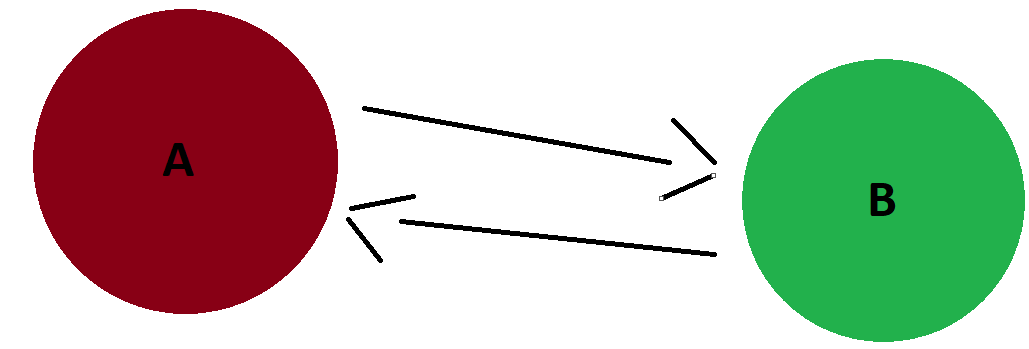
\includegraphics[width = \linewidth]{Billeder/damping_fac.png}
    \caption{Illustration af det beskrevne nedenunder. Udarbejdet af os.}
    \label{fig:my_label}
\end{figure}

Når man går ind på en hjemmeside vil der oftest være såkaldte hyperlinks der tager brugeren til en anden hjemmeside. Lad os betragte en situation hvor en hjemmeside A kun linker til en hjemmeside B og hjemmeside B kun linker til hjemmeside A. Når dette er tilfældet, og man kører vores algoritme vil man jo netop sidde fast ved disse to hjemmesider under hele forløbet, og således vil det være vanskeligt at bestemme en "ordentlig"  PageRank. For at undgå dette har vi en såkaldt dæmpningsfaktor, $d$ (eng.: damping factor). Formålet med denne er at give en mulighed for at dæmpe algortimen ved algoritmens næste skridt. Dette skal forstås således: Enten udvælges et tilfældigt hyperlink på den nuværende hjemmeside eller udvælges en tilfældig hjemmeside i vores sæt af hjemmesider ($W$). En almindelig værdi for $d$ er 0.85, dvs. 85\% sandsynlighed for at udvælge et tilfældigt hyperlink som hjemmeside $P_i$ linker til og $1 - d = 0.15$ dvs. 15\% sandsynlighed for at udvælge en tilfældig hjemmeside i sættet $W$ (nuværende hjemmeside inkluderet).

\subsection*{Random Surfer Model}
For at videreuddybe konceptet beskrevet foroven: Vi har et sæt af hjemmesider, $W$, hvorledes der er $N$-antal hjemmesider. For hver (men ikke nødevendigvis alle) hjemmeside $P_i$ er der et vis antal hyperlinks der fører videre til en anden hjemmeside. Dette er det grundlæggende for at kunne bestemme det såkaldte PageRank. En metode til denne algoritme er \emph{Random Surfer Model}, hvor der indledningsvist udvælges en tilfældig hjemmeside i sættet $W$, dvs. hver hjemmeside har sandsynligheden $\frac{1}{n}$ for at bliver udvalgt. Her vil modellen således udvælge et tilfældigt hyperlink på den nuværende hjemmeside $P_i$, hvor hvert besøg hos hjemmesiden bliver talt. Hvis modellen er kørt $n$-gange og en hjemmeside $P_k$ er blevet besøgt $N_k$ gange vil $\frac{N_k}{n}$ således være sandsynligheden for at ankomme på hjemmesiden tilfældigt. Og i teorien hvis dette kører nok gange (hvis $n \rightarrow \infty$, eller hvis det måles i tid $t \rightarrow \infty$) vil dette netop være hjemmesidens $P_k$ såkaldte PageRank. Dæmpningsfaktoren kommer i spil netop der hvor modellen udvælger et tilfældigt hyperlink på nuværende hjemmeside $P_i$, som beskrevet i afsnittet "Dæmnpningsfaktor". Dette er jo som sagt for at bekæmpe instanser hvor en hjemmeside er et såkaldt "sink" (ingen hyperlinks) eller hvis to hjemmesider kun fører til hinanden.


\subsection*{title}

\subsection*{Beskrivelse af programmet}

\subsection*{Tilgange til projektet}

\subsection*{Illustrationer og eksempler}